\normaltrue
\correctionfalse

%\UPSTIidClasse{12} % 11 sup, 12 spé
%\newcommand{\UPSTIidClasse}{12}

\exer{Banc d'épreuve hydraulique $\star$ \label{C2:09:1D:63_02}}
\setcounter{numques}{0}
\UPSTIcompetence[2]{C2-09}
\index{Compétence C2-09}
\index{Principe fondamental de la dynamique}
\index{PFD}
%\index{Mécanisme à 1 rotation}
\index{Banc d'épreuve hydraulique} % CCP PSI 2010
\ifcorrection
\else
\textbf{Pas de corrigé pour cet exercice.}
\fi



Le multiplicateur, représenté fiugure suivante, se compose d’un piston, de masse $M$, en translation par rapport au bâti, séparant les chambres $C_e$ et $C_h$ comportant respectivement de l’eau et de l’huile sous pression :
On note :
\begin{itemize}
\item $Q_e(t)$ : le débit volumique d’eau en sortie du multiplicateur;
\item $Q_h(t)$ : le débit volumique d’huile en entrée du multiplicateur;
\item $P_e(t)$ : la pression d’eau dans $C_e$;
\item $P_h(t)$ : la pression d’huile dans $C_h$;
\item $z(t)$ : la position du piston;
\item $V_e(t)$ : le volume de $C_e$;
\item $V_h(t)$ : le volume de $C_h$;
\item $g$ : l’accélération de pesanteur;
\item $\vect{z}$ : le vecteur vertical unitaire ascendant.
\end{itemize}

Les équations du débit sont :
\begin{itemize}
\item $\quad Q_e (t)=S_e\dfrac{\dd z(t)}{\dd t}-\dfrac{V_{e0}}{B_e}  \dfrac{\dd P_e (t)}{\dd t}$;
\item $\quad Q_h (t)=S_h\dfrac{\dd z(t)}{\dd t}+\dfrac{V_{h0}}{B_h}  \dfrac{\dd P_h (t)}{\dd t}$x
\end{itemize}




\begin{figure}[H]
\centering
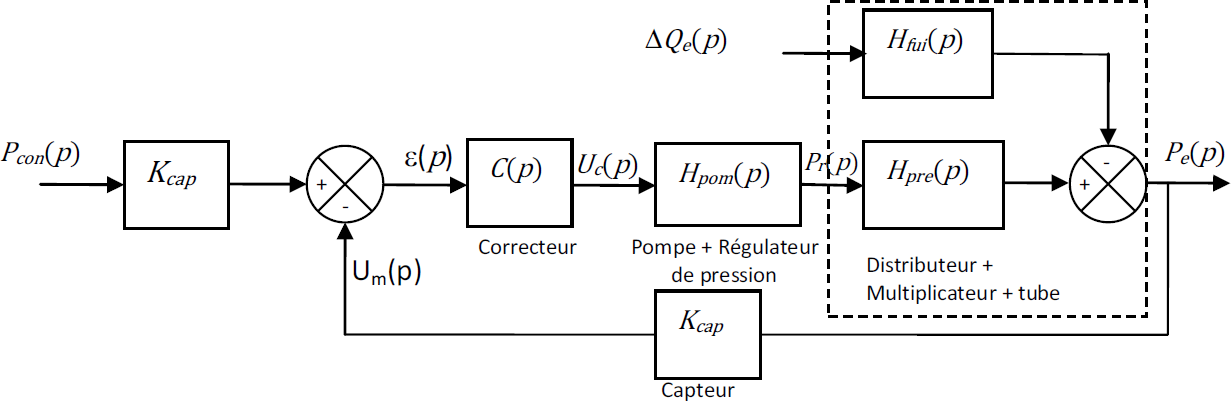
\includegraphics[width=\linewidth]{63_01}
%\caption{\label{61_01} Loi de commande de vitesse en trapèze}
\end{figure}


%
%\question{Les conditions initiales étant supposées nulles, transposer les équations du débit dans le domaine de Laplace}
%\ifprof
%\else
%\fi

\question{En appliquant le théorème de la résultante dynamique selon $\vect{z}$  sur le piston du multiplicateur, déterminer son équation du mouvement et en déduire l’équation reliant $Z(p)$, $P_e(p)$,  $P_h(p)$, et $\text{Poids}(p)=\dfrac{Mg}{p}$, transformées de Laplace de $z(t)$, $P_e(t)$, $P_h(t)$ et du poids perçu comme une perturbation. Les conditions initiales sont supposées nulles.}
\ifprof
\else
\fi


Le chariot avant comporte  :
\begin{itemize}
\item la traverse, mise en position par un vérin hydraulique avant la mise sous pression du tube. Durant toute la durée de l’épreuve, on supposera que la traverse est immobile par rapport au bâti.
\item un équipage mobile sur lequel est monté l’outillage, en translation rectiligne par rapport à la traverse.
\end{itemize}


On note :
\begin{itemize}
\item $L(t)$ : la position de l’équipage mobile repérée par rapport à sa position initiale
\item $V_t(t)$ : le volume du tube
\item $F_t(t)$ : l’effort du tube sur l’équipage mobile, avec $F_t(t) = - r.L(t)$.
\end{itemize}
On néglige les variations de volume du tube dues à ses déformations. L’équation du débit s’écrit alors :
$Q_e (t)=(S_a-S_b ) \dfrac{dd L(t)}{\dd t}+\dfrac{V_t}{B_e}\dfrac{\dd dP_e (t)}{\dd t}$.

\question{Ecrire l’équation du mouvement de l’équipage mobile. En déduire, en tenant compte de l’équation précédente, deux équations liant $L(p)$, $P_e(p)$ et $Q_e(p)$, transformées de Laplace de $L(t)$, $P_e(t)$ et $Q_e(t)$. Les conditions initiales sont supposées nulles.}
\ifprof
\else
\fi



\begin{figure}[H]
\centering
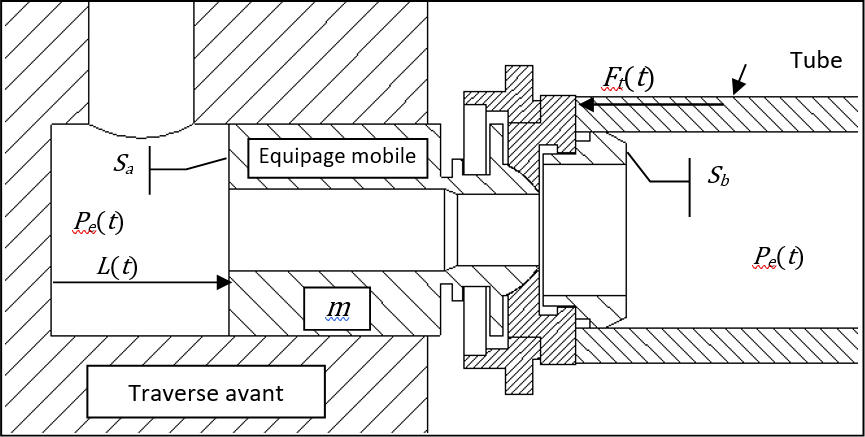
\includegraphics[width=\linewidth]{63_02}
%\caption{\label{61_01} Loi de commande de vitesse en trapèze}
\end{figure}


\ifprof

\else
\footnotesize
\begin{enumerate}
  \item $\left(fp + Mp^2\right) Z(p)=S_h P_h(p)-S_e P_e(p) - \dfrac{Mg}{p}$
    \item $Q_e(p)=\left(S_a - S_b \right)pL(p) + \dfrac{V_t}{B_e} p P_e(p)$ et $mp^2 L(p) = -rL(p)+\left(S_a-S_b\right) P_e(t)-f'pL(p)$.
\end{enumerate}
\normalsize

\begin{flushright}
\footnotesize{Corrigé  voir \ref{C2:09:1D:63_02}.}
\end{flushright}%
\fi